\documentclass[a4paper,11pt]{article}
\usepackage{graphicx}
\usepackage{amsmath}
\usepackage{hyperref}
\usepackage{geometry}
\usepackage{natbib}
\usepackage{project}
\usepackage{tikz}
\usetikzlibrary{positioning, shapes.geometric, arrows}
\setlength{\headheight}{13.6pt}

\begin{document}

\section{Questions}
    \begin{itemize}
        \item How does neighborhood poverty level impact school enrollment rates across different regions in the United States?
    
        \item How do poverty levels around schools vary by region in the United States, and what might these differences suggest about educational inequality?
    \end{itemize}

\section{Data Sources}
    \subsection{Description of Data Sources}
        \begin{itemize}
            \item \textbf{Dataset 1: School Neighborhood Poverty Estimates 2020-2021}
    
            This datset from the National Center for Education Statistics \(\text(NCES)\) includes data on neighborhood poverty levels surrounding schools, which can serve as a proxy for educational access and community socioeconomic conditions. \cite{dataset1}

            \item \textbf{Dataset 2: Report Card Enrollment}

            This dataset provides detailed school enrollment statistics disaggregated by school, district, and state for the 2022-23 school year. It includes student counts by demographics, which can help analyze how regional poverty levels might influence enrollment and highlight disparities across regions. \cite{dataset2}
        \end{itemize}

    \subsection{Data Structure and Quality}
        \begin{itemize}
            \item \textbf{School Neighborhood Poverty Estimates 2020-2021} 
            \begin{figure}[ht!]
                \centering
                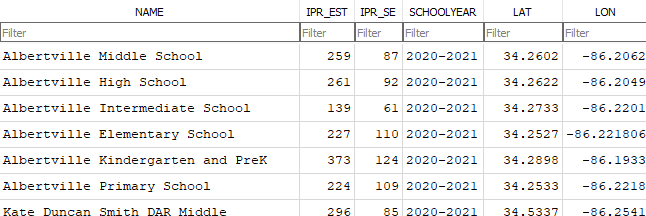
\includegraphics[width=0.9\textwidth]{images/SchoolNeighborhoodPovertyData.png}
                \caption{School neighborhood poverty estimate 2020-2021 dataset}
                \label{fig:dataset1}
            \end{figure}
            
            The data is organized with geospatial data (latitude and longitude) defining the locations of various education systems. It also includes the income-to-poverty ratio (IPR) which measure the socioeconomics conditions in surroundings to the schools. Additionally, It defines the standard error of the IPR for each area.
            
\newpage
            \item \textbf{Report Card Enrollment} 
            \begin{figure}[h!]
                \centering
                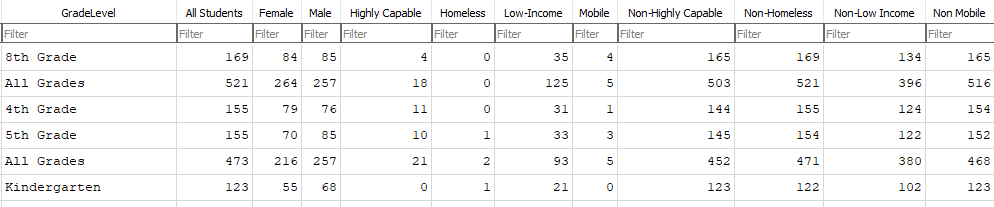
\includegraphics[width=0.9\linewidth]{images/ReportCardEnrollmentData.png}
                \caption{Report card Enrollment}
                \label{fig:dataset2}
            \end{figure}
        \end{itemize} The data is structured for analyzing school-specific or regional educational trends. Mainly it contains the statistical metrics of enrollment in different Education system. Also, providing the income category by which students are belonging. 

    \subsection{Licenses and Permissions}
        The data sources are publicly available on under \href{https://catalog.data.gov//}open-data licenses. Detailed license information can be found at \href{https://resources.data.gov/open-licenses/}{License}
    
\section{Data Pipeline}
    The data pipeline engineering is designed and developed with python has three main modules: extractor, transform, and loader, each module contains respective functionalities. Furthermore, the pipeline helper has responsibility to initialize the desire configuration for data sources.

    After configuration Initialization for data sources, each module perform its responsibility. First \texttt{extract} from extractor module is used to extract the data source from url, second \texttt{delete\_columns} from transform module deletes the list of useless columns specified for every dataset. Additionally, eradicate the rows contain null or empty record, once all the transformations have been applied, dataset is then loaded to sqlite database using \texttt{load\_df\_to\_sqlite} from loader module.

    \begin{figure}[h]
        \centering
        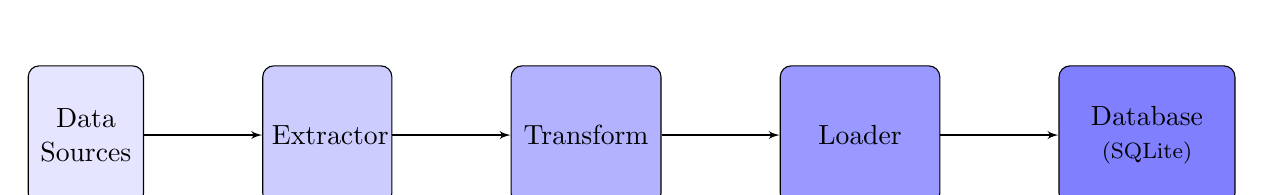
\begin{tikzpicture}[node distance=1cm and 1.5cm, auto]
            \tikzstyle{datasource} = [rectangle, draw, fill=blue!10,
                text width=3.5em, text centered, rounded corners, minimum height=5em]
            \tikzstyle{E} = [rectangle, draw, fill=blue!20,
                text width=4em, text centered, rounded corners, minimum height=5em]
            \tikzstyle{T} = [rectangle, draw, fill=blue!30,
                text width=4.75em, text centered, rounded corners, minimum height=5em]
            \tikzstyle{L} = [rectangle, draw, fill=blue!40,
                text width=5.1em, text centered, rounded corners, minimum height=5em]
            \tikzstyle{db} = [rectangle, draw, fill=blue!50,
                text width=6em, text centered, rounded corners, minimum height=5em]
            \tikzstyle{line} = [draw, -latex', shorten >=0pt, shorten <=0pt]

            \node [datasource] (source) {Data Sources \\ \footnotesize};
            \node [E, right=of source] (extractor) {Extractor};
            \node [T, right=of extractor] (transform) {Transform};
            \node [L, right=of transform] (loader) {Loader};
            \node [db, right=of loader, text width=2cm, align=center] (database) {Database \\ \footnotesize (SQLite)};

            \path [line] (source) -- (extractor);
            \path [line] (extractor) -- (transform);
            \path [line] (transform) -- (loader);
            \path [line] (loader) -- (database);
        \end{tikzpicture}
    \caption{ETL Pipeline Flow}
    \label{fig:etl}
    \end{figure}

\section{Result and Limitations}
    The pipeline stored an output in SQLite database in table format. This is one of the fastest and easier method to deal with the data. The pipeline is smart-enough
    to maintain the stored data quality.
    \begin{itemize}
        \item All necessary information is available to support the analysis questions.
        \item The data is consistent in their formats.
        \item The data reflects the real word and are correct indicators.
    \end{itemize}

\bibliographystyle{plain}
\bibliography{reference}
\end{document}